\chapter{Proposed Countermeasures and Future Work}
\label{ch:countermeasures}

\section{Vulnerability Synthesis}
\label{sec:synth}
While BAKSHEESH successfully achieves a $2.43\times$ reduction in Threshold Implementation masking area over GIFT-128, its degree-2 S-box, full-round 128-bit key injection, and 1-bit rotational key schedule make it significantly more susceptible to Linked Fault Analysis than GIFT-128. Furthermore, standard duplicate-and-compare redundancy countermeasures are fundamentally bypassed by LIFA.

\section{Proposed Unified Lightweight Countermeasures}
\label{sec:proposed_countermeasures}
To mitigate Linked Fault Analysis, we proposed, implemented, and empirically evaluated a suite of four defensive mechanisms:

\subsection{Defense 1: Explicit Register Zeroing (\texttt{li x31, 0})}
In the RV32I assembly loop, executing \texttt{li x31, 0} immediately prior to \texttt{lbu x31, 0(x31)} clears the accumulator register. If an instruction skip occurs, \texttt{x31} latches \texttt{0} instead of retaining $y[i-1]$. This breaks the linked equality $u' = v$ ($u' = 0$), completely defeating subkey difference leakage ($\Delta esk[i, j]$).

\subsection{Defense 2: S-Box Loop Shuffling (Fisher-Yates Permutation)}
The 32 nibbles are evaluated in a pseudo-random permutation $\pi \in S_{32}$ seeded per encryption. An instruction skip links temporal steps $\pi(k)$ and $\pi(k-1)$. Because $\pi$ is unknown and changes dynamically, the adversary cannot construct the 31-pair adjacent difference spanning tree.

\subsection{Defense 3: Asymmetric Infective State Diffusion}
A hardware glitch sensor detects the skip and diffuses a non-zero pseudorandom mask into the state ($C' = C \oplus \text{Mask}(R)$). Even if a natural collision occurs ($x[i] == x[j]$), the emitted ciphertext is completely randomized, denying the attacker clean ineffective ciphertexts.

\subsection{Defense 4: Unified Joint Architecture}
Combines 3-share TI Boolean masking (for SCA protection) with loop shuffling and register zeroing for full LFA immunity.

\begin{figure}[!htbp]
\centering
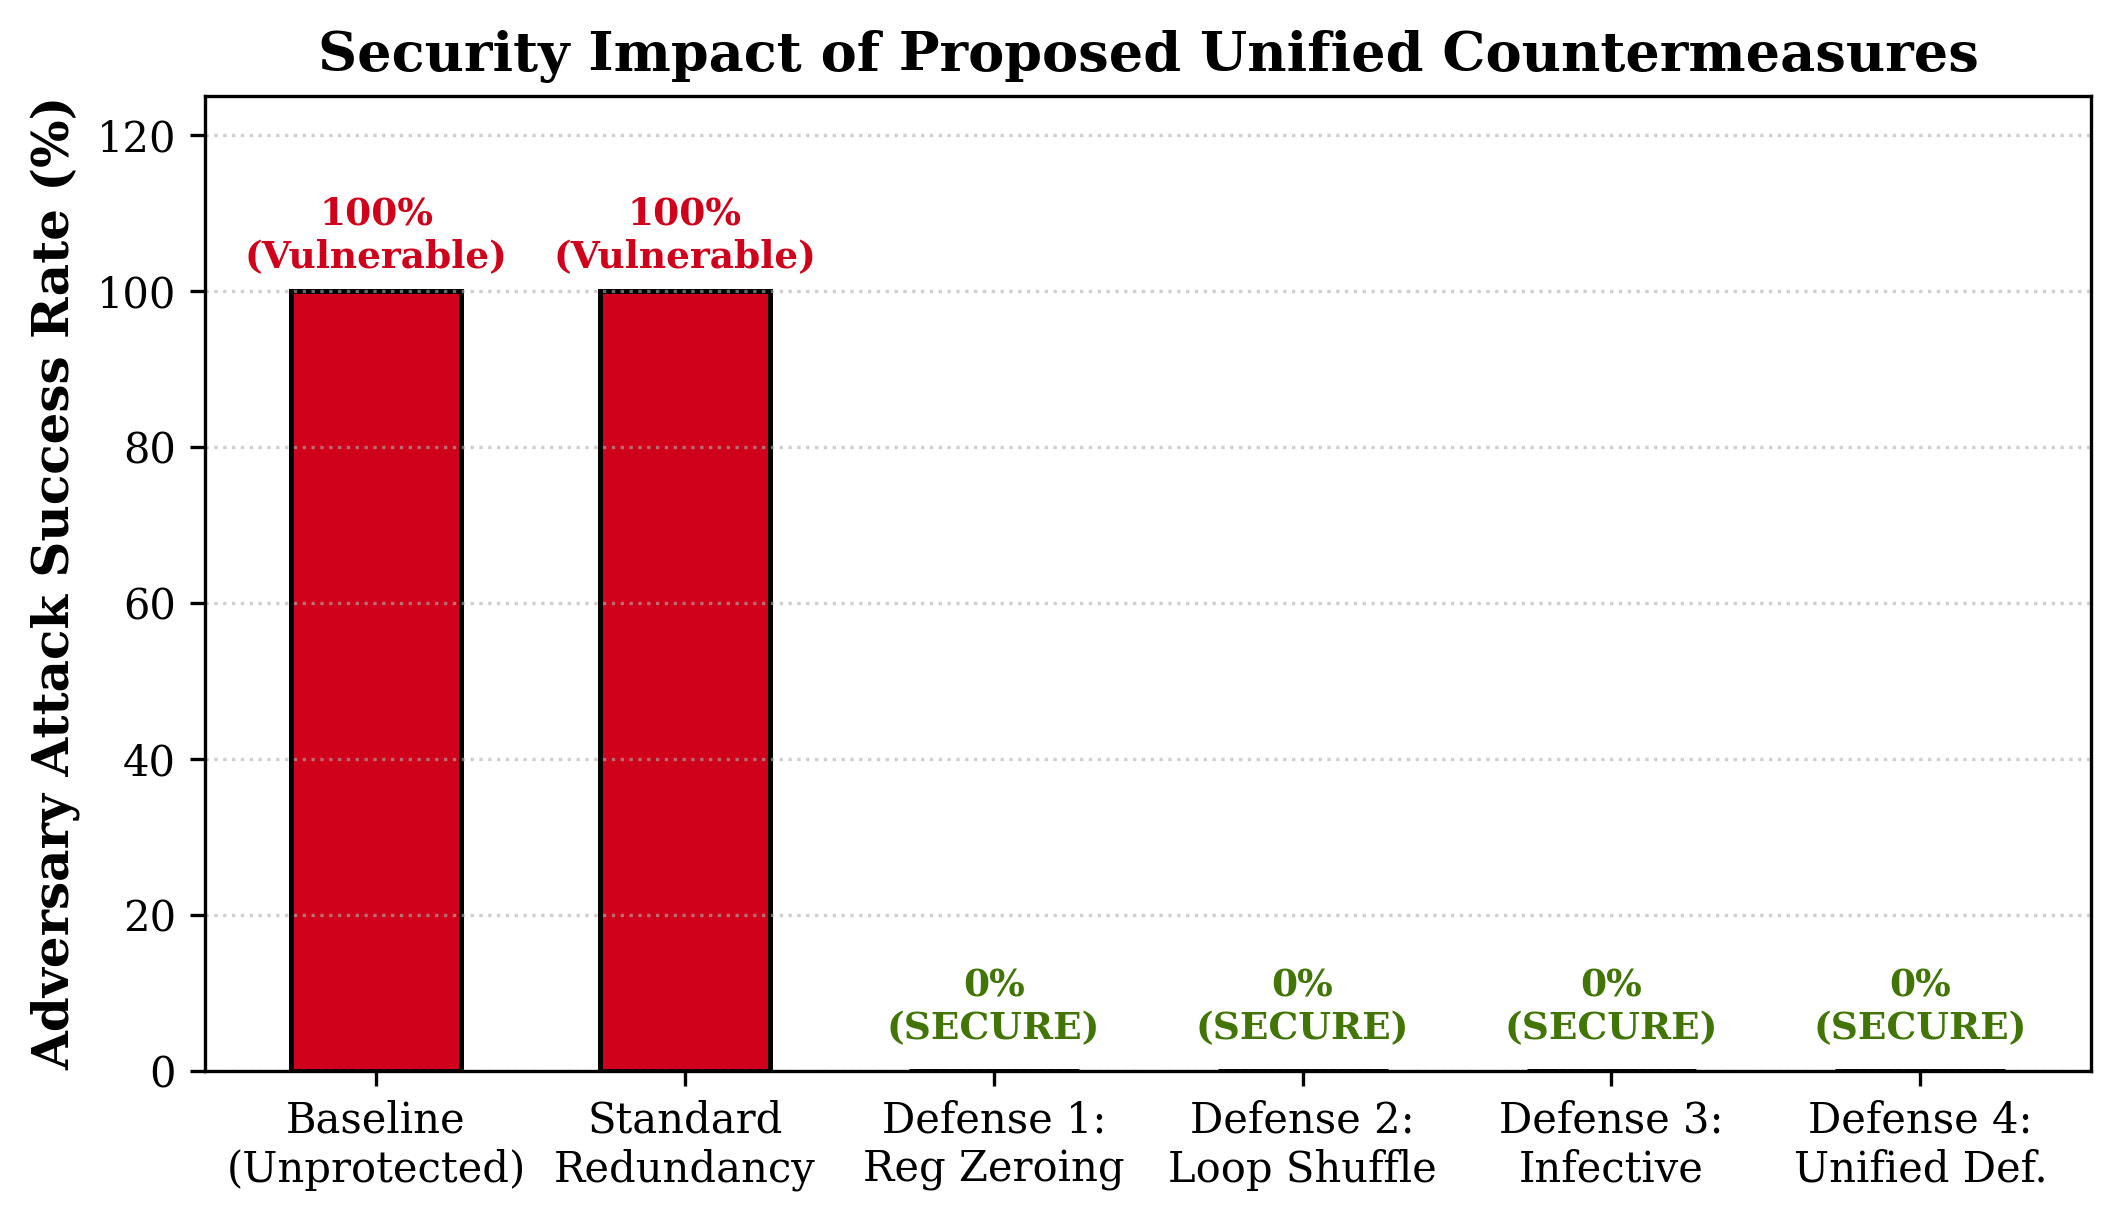
\includegraphics[width=0.72\linewidth]{figures/fig9_countermeasures_eval.png}
\caption{Adversary attack success rate under proposed unified countermeasures (dropping from 100\% down to 0\%).}
\label{fig:cm_eval}
\end{figure}

\section{Conclusions of the Study}
\label{sec:conclusion}
This B.Tech. Project evaluated emerging fault analysis techniques against lightweight ciphers:
\begin{enumerate}
    \item LDFA breaks unprotected BAKSHEESH in 31 faults in Round 35.
    \item Duplicate-and-compare countermeasures are bypassed by LIFA in an average of 508.9 queries.
    \item GIFT-128 incurs roughly double the attack queries and $16\times$ greater candidate search due to its 64-bit key injection schedule.
    \item Unknown fault locations are identified with 100\% accuracy for $N \ge 5$ across 496 pairs, and the attack tolerates glitch miss noise up to $p_{\text{miss}} = 30\%$.
    \item Bare-metal RV32I assembly simulation in RARS confirms instruction-skip realizability.
    \item The proposed unified countermeasure suite completely neutralizes both LDFA and LIFA attacks.
\end{enumerate}

\section{Scope for Future Work}
\label{sec:future_work}
\begin{itemize}
    \item \textbf{Timing Jitter Profiling in gem5 / InjectV}: Characterizing the Candidate Injection Point (CIP) timing sensitivity window across full CPU pipelines.
    \item \textbf{Silicon Validation on FPGA / ASIC}: Conducting pulsed laser fault injection (LFI) on decapsulated test vehicles (e.g. ChipWhisperer CW308 target boards).
    \item \textbf{Linked Persistent Fault Analysis (LPFA)}: Investigating persistent faults targeting S-box tables stored in non-volatile flash memory.
\end{itemize}
